% Name: Function on coordinate axes
% Description: A cubic on a grid with tick marks, labels, and its two turning points marked.
% Tags: function, graph, axes, plot

\usetikzlibrary{arrows.meta}

\begin{tikzpicture}[>={Stealth}]
  \draw[gray!20] (-3,-2) grid (3,2);
  \draw[->] (-3.2,0) -- (3.3,0) node[right] {$x$};
  \draw[->] (0,-2.2) -- (0,2.4) node[above] {$y$};
  \foreach \x in {-3,-2,-1,1,2,3}
    \draw (\x,0.08) -- (\x,-0.08) node[below, font=\footnotesize] {$\x$};
  \foreach \y in {-2,-1,1,2}
    \draw (0.08,\y) -- (-0.08,\y) node[left, font=\footnotesize] {$\y$};
  \draw[very thick, blue!70!black, domain=-2.3:2.3, samples=80, smooth]
    plot (\x, {\x*\x*\x/3 - \x});
  \fill[orange!85!black] (-1,2/3) circle (2pt) (1,-2/3) circle (2pt);
  \node[blue!70!black, fill=white, inner sep=2pt] at (-1.9,1.6) {$f(x) = \tfrac{1}{3}x^3 - x$};
\end{tikzpicture}
